\documentclass[conference]{IEEEtran}
\IEEEoverridecommandlockouts
\usepackage{amsmath,amssymb,amsfonts}
\usepackage{algorithm}
\usepackage{algorithmic}
\usepackage{graphicx}
\graphicspath{{images/}}
\usepackage{textcomp}
\usepackage{xcolor}
\usepackage{booktabs}
\usepackage{array}
\usepackage{url}
\usepackage{cite}
\usepackage[compact]{titlesec}
\titlespacing{\section}{0pt}{6pt plus 2pt minus 2pt}{3pt plus 1pt minus 1pt}
\titlespacing{\subsection}{0pt}{4pt plus 2pt minus 2pt}{2pt plus 1pt minus 1pt}
\usepackage{tikz}
\usetikzlibrary{arrows.meta,positioning,shapes.geometric}

\setlength{\textfloatsep}{4pt plus 1pt minus 1pt}
\setlength{\dbltextfloatsep}{4pt plus 1pt minus 1pt}
\setlength{\intextsep}{4pt plus 1pt minus 1pt}
\setlength{\abovecaptionskip}{2pt plus 1pt minus 1pt}
\setlength{\belowcaptionskip}{2pt plus 1pt minus 1pt}

\def\BibTeX{{\rm B\kern-.05em{\sc i\kern-.025em b}\kern-.08em
    T\kern-.1667em\lower.7ex\hbox{E}\kern-.125emX}}

\begin{document}

\title{
\textbf{Application of TCN and Transformer Networks for Log Anomaly Detection in Large-Scale Enterprise and Industrial Networks}\\[0.8em]
}

\author{\IEEEauthorblockN{Hoang-Tu Trinh\thanks{The complete source code and raw training logs to ensure experiment reproducibility are publicly available at: \protect\url{https://github.com/thtcsec/vnict2026-log-anomaly}.}}
\IEEEauthorblockA{\textit{Department of Information Technology} \\
\textit{Ho Chi Minh City University of} \\
\textit{Foreign Languages - Information Technology} \\
\textit{(HUFLIT)}\\
Ho Chi Minh City, Vietnam \\
Email: tht.csec2005@gmail.com}
\and
\IEEEauthorblockN{Tien-Thanh Cao}
\IEEEauthorblockA{\textit{Department of Information Technology} \\
\textit{Ho Chi Minh City University of} \\
\textit{Foreign Languages - Information Technology} \\
\textit{(HUFLIT)}\\
Ho Chi Minh City, Vietnam \\
Email: thanhct@huflit.edu.vn}
}

\maketitle

\begin{abstract}
This paper presents a large-scale system log anomaly detection pipeline based on Drain3 and event sequence analysis, comparing Temporal Convolutional Networks (TCN) and Transformers against traditional baselines on two large-scale enterprise and industrial network log datasets. Raw logs are parsed into event templates, grouped into sequences, and scored for anomalies using five branches: PCA/SVD, Isolation Forest, DeepLog (LSTM next-event prediction), TCN (Temporal Convolutional Network), and Transformer masked event modeling. On HDFS (500k lines, 137 templates), experiments across 5 random seeds show that PCA achieves an F1-score of $0.5711 \pm 0.0944$, slightly outperforming DeepLog and TCN ($0.4613 \pm 0.0199$). On BGL (500k lines, 198 templates, window size $W{=}100$), TCN leads with an F1-score of $0.9826 \pm 0.0022$ (top-k mode) and $0.9474 \pm 0.0035$ (NLL threshold mode), outperforming DeepLog LSTM ($0.9820 \pm 0.0042$ and $0.9381 \pm 0.0075$) as well as the val-tuned Transformer ($0.9388 \pm 0.0080$). The results demonstrate that TCN has a significant advantage in both classification performance and inference latency compared to LSTM and Transformer models on long sequences. The contributions include: (i) a reproducible evaluation pipeline that prevents data leakage; (ii) an ablation study on Drain3 similarity threshold, DeepLog/TCN top-k, and Transformer mask ratio; (iii) a cross-dataset evaluation between HDFS and BGL; (iv) an inference latency benchmark of TCN and Transformer on CPU.
\end{abstract}

\begin{IEEEkeywords}
Log anomaly detection, masked event modeling, Transformer, Drain3, AIOps, distributed systems.
\end{IEEEkeywords}

\section{Introduction}
Modern large-scale enterprise and industrial network infrastructures integrate web servers, databases, distributed storage services, authentication systems, APIs, and cloud services; each component generates logs with different formats and frequencies. System logs reflect both the technical state and specific business workflows, such as batch logins, file system access, and service API calls, while manual rules quickly become outdated as the system evolves. Log anomaly detection therefore needs to be processed at the event sequence level rather than individual log lines.

This paper is positioned as an applied research and system evaluation study, rather than proposing a new anomaly detection algorithm. The central idea is to treat the event template sequence after Drain3 parsing as an intermediate representation layer: compact enough to run lightweight baselines, structured enough to extend to sequence models, and clear enough to map to operational units such as sessions, anonymized users, or time windows. Three research questions are addressed:
\begin{itemize}
    \item \textbf{RQ1:} How does the method of constructing event sequences after Drain3 affect the anomaly detection signal?
    \item \textbf{RQ2:} How do the four scoring branches (reconstruction, isolation, next-event, masked event modeling) perform differently on the same event sequence?
    \item \textbf{RQ3:} Does the performance ranking of these branches remain consistent when moving from HDFS to BGL (datasets with very different characteristics)?
\end{itemize}

The main contributions include: (1) an end-to-end pipeline of Drain3 parsing, event sequencing, and anomaly scoring with four alternative branches (PCA/SVD, Isolation Forest, DeepLog, and Transformer masked event modeling); (2) a multi-seed evaluation (5 random seeds) on HDFS with a protocol that prevents test set leakage, along with a grouping strategy study for Block ID, fixed window, and sliding window; (3) a cross-dataset HDFS-BGL evaluation on the same pipeline; (4) an ablation study for Drain3 threshold, DeepLog top-k, and Transformer mask ratio, and an inference latency benchmark; (5) a cost analysis, expected error analysis, and cautious mapping to large-scale network infrastructures.

\section{Related Work}
The earliest log anomaly detection methods typically represented log data as event count vectors or feature matrices, and then applied traditional machine learning models such as PCA, clustering, or Isolation Forest \cite{b10,b11}. PCA is used to separate normal behavior space and detect points deviating from the principal subspace. This group of methods is lightweight and easy to deploy, but usually ignores the temporal order and contextual relationships between log events.

To address this limitation, sequential models like DeepLog \cite{b1} use LSTM networks to predict the next event based on previous events. LogAnomaly \cite{b13} and LogRobust \cite{b14} extend this direction by combining sequential and semantic log information to deal with unstable log data. Additionally, semi-supervised approaches such as PLELog \cite{b15} use probabilistic label estimation to reduce dependence on manual labels. Overall, RNN/LSTM architectures capture sequence relationships better than traditional statistical methods, but still suffer from sequential processing limitations and are difficult to parallelize.

To represent unstructured logs for machine learning models, log parsing techniques are used to map each log line to a template. Drain \cite{b3} and Drain3 are widely used due to their fixed-depth parse tree structure, which allows high-speed online parsing. Recently, LogPPT \cite{b7} used prompt-based few-shot learning to improve parsing accuracy when labeled data is scarce.

The Transformer architecture with its self-attention mechanism \cite{b4} has been widely applied in AIOps. LogBERT \cite{b2} employs a Transformer encoder combined with masked event modeling to learn bidirectional representations for normal log sequences, improving contextual anomaly detection. Survey papers also note a strong shift from traditional sequential models to self-supervised deep learning based on Transformers \cite{b16}. In parallel, Large Language Model (LLM) and prompt learning approaches such as LogPrompt \cite{b8} and LogGPT \cite{b9} enhance semantic understanding, but face major barriers in terms of inference cost and real-time latency.

\begin{table}[htbp]
\caption{Comparison of methodology groups and research gaps}
\begin{center}
\scriptsize
\setlength{\tabcolsep}{3pt}
\begin{tabular}{lp{1.6cm}p{2.3cm}p{2.1cm}}
\toprule
\textbf{Group} & \textbf{Representatives} & \textbf{Key Limitation} & \textbf{Improvement in This Work} \\
\midrule
Statistical & PCA, IF \cite{b10,b11} & No temporal ordering & Lightweight baseline quantification \\
Sequential & DeepLog \cite{b1,b13} & Limited sequence length, sequential bottleneck & Parallel TCN integration \\
Transformer & LogBERT \cite{b2} & Dependent on parsing quality & Decoupled parsing, grouping, and scoring \\
\bottomrule
\end{tabular}
\label{tab_related_work}
\end{center}
\end{table}

From existing works, four main research gaps can be identified: (i) traditional statistical methods do not learn the order of log events; (ii) sequential LSTM models are limited with long log sequences; (iii) Transformer models depend heavily on the parsing step; (iv) mapping anomaly detection pipelines to large networks requires clarifying the grouping strategy and business scenarios. 

To address these gaps, this paper builds a standardized pipeline that separates three phases (parsing, grouping, and scoring) using Drain3 as a preprocessing step to clean the token space. We evaluate in parallel the scoring branches including lightweight baselines (PCA, TruncatedSVD, Isolation Forest), sequential LSTM (DeepLog), the proposed Temporal Convolutional Network (TCN), and Transformer masked event modeling. Performance is carefully measured using Precision, Recall, and F1-score averaged over 5 different random seeds to ensure scientific reliability. To ensure experiment reproducibility and verification, the complete source code and raw training logs are publicly available at \url{https://github.com/thtcsec/vnict2026-log-anomaly}.

\section{Proposed Methodology}
\subsection{Pipeline Overview}
The proposed pipeline is designed to clearly separate three processing layers: log standardization, event sequence construction, and anomaly detection. The input is a raw log dataset $L=\{l_1,l_2,\ldots,l_N\}$ generated from the operating system. The output is an anomaly label or score $a(S)$ for each event sequence $S$. In HDFS experiments, a sequence corresponds to a Block ID; in large-scale enterprise and industrial network environments, a sequence can correspond to a login session, an anonymized user, a service, or a time window.

\begin{figure}[!t]
\centering
\resizebox{0.9\columnwidth}{!}{
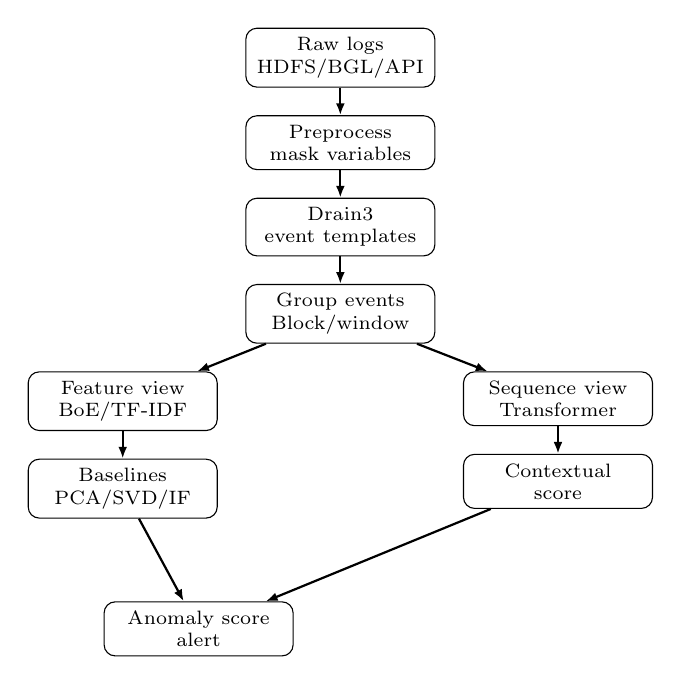
\begin{tikzpicture}[
    node distance=0.35cm and 0.35cm,
    box/.style={rectangle, draw, rounded corners, align=center, minimum width=2.4cm, minimum height=0.5cm, font=\scriptsize},
    arrow/.style={-{Latex[length=1.5mm]}, thick}
]
\node[box] (raw) {Raw logs\\HDFS/BGL/API};
\node[box, below=of raw] (pre) {Preprocess\\mask variables};
\node[box, below=of pre] (parse) {Drain3\\event templates};
\node[box, below=of parse] (seq) {Group events\\Block/window};
\node[box, below left=of seq] (vec) {Feature view\\BoE/TF-IDF};
\node[box, below=of vec] (base) {Baselines\\PCA/SVD/IF};
\node[box, below right=of seq] (bert) {Sequence view\\Transformer};
\node[box, below=of bert] (seqscore) {Contextual\\score};
\node[box, below right=1.05cm and -1.45cm of base] (score) {Anomaly score\\alert};
\draw[arrow] (raw) -- (pre);
\draw[arrow] (pre) -- (parse);
\draw[arrow] (parse) -- (seq);
\draw[arrow] (seq) -- (vec);
\draw[arrow] (vec) -- (base);
\draw[arrow] (seq) -- (bert);
\draw[arrow] (bert) -- (seqscore);
\draw[arrow] (base) -- (score);
\draw[arrow] (seqscore) -- (score);
\end{tikzpicture}
}
\caption{Proposed log anomaly detection pipeline block diagram}
\label{fig_pipeline}
\end{figure}

The overall process consists of six steps:
\begin{itemize}
    \item \textbf{Step 1 -- Log Collection:} receive logs from source systems such as HDFS, BGL, API gateways, or authentication servers.
    \item \textbf{Step 2 -- Preprocessing:} normalize variable fields such as timestamps, IPs, user IDs, session IDs, and query parameters.
    \item \textbf{Step 3 -- Log Parsing:} use Drain3 to map each log line to an event template and event ID.
    \item \textbf{Step 4 -- Event Grouping:} group event IDs by Block ID or by session/time window to create event sequences.
    \item \textbf{Step 5 -- Feature Representation:} generate bag-of-events/TF-IDF representation for baselines or keep the raw event sequence for Transformer masked event modeling.
    \item \textbf{Step 6 -- Anomaly Detection:} compute anomaly scores using reconstruction error, Isolation Forest, or sequence learning models.
\end{itemize}

In large-scale enterprise and industrial networks, this pipeline can be adapted to other sources such as application servers, API gateways, reverse proxies, authentication systems, and databases after anonymizing the logs. Instead of building specific rules for each log source, the system learns normal operational patterns from event sequences and flags sequences that deviate from these patterns. This generalizability needs to be confirmed with real system logs in future work.

\subsection{Preprocessing, Drain3 Parsing, and Event Grouping}
The input is a raw log set $L=\{l_1,l_2,\ldots,l_N\}$. The process consists of: (i) normalizing variable parameters (IP, timestamp, ID); (ii) parsing raw logs into event templates using Drain3 \cite{b3}; (iii) grouping event IDs into sequences by Block ID or time windows.

Drain3 uses a fixed-depth tree to find the corresponding event template for each log line. The similarity between two log lines $T_1, T_2$ is calculated as the ratio of matching tokens:
\begin{equation}
Sim(T_1, T_2) = \frac{1}{n} \sum_{i=1}^{n} equ(t_{1,i}, t_{2,i})
\label{eq_sim}
\end{equation}
If $Sim(T_1, T_2) > st$ (similarity threshold, default 0.5), the log line is assigned to an existing template; otherwise, Drain3 creates a new template. After this step, each template is assigned an event ID, and the log sequence is represented as:
\begin{equation}
S = [E_1, E_2, ..., E_m]
\end{equation}
For HDFS, the sequence $S$ is grouped by Block ID. For BGL, it is grouped by non-overlapping windows of $W{=}100$ lines. We also support sliding window strategies to study the effect of the grouping strategy.

\subsection{Lightweight Machine Learning Baselines}
PCA and TruncatedSVD are applied to the bag-of-events vector representation $x = [count(E_j, S)]_{j=1}^d$ to learn the normal behavior subspace. The anomaly score is computed as the reconstruction error:
\begin{equation}
score(S)=\frac{1}{d}\sum_{j=1}^{d}(x_j-\hat{x}_j)^2
\label{eq_reconstruction}
\end{equation}
where $\hat{x}$ is the reconstructed vector after projecting onto the low-dimensional space (the number of principal components is set to 20 by default). The anomaly threshold $\tau$ is chosen as the 95th percentile on the normal training set. A sequence $S$ is labeled as anomalous if $score(S) > \tau$.
Isolation Forest is applied to the TF-IDF feature representation of the event sequences. The model isolates sparse data points using random partitioning trees.

\subsection{Deep Sequence Models and Transformer}
\textbf{DeepLog (LSTM):} Replicated as next-event prediction using a 2-layer LSTM \cite{b1}. For each position $i$, the model predicts the probability of event $E_i$ given the context of the previous $g$ events:
\begin{equation}
\hat{P}(E_i \mid E_{i-g}, \ldots, E_{i-1}) = \text{softmax}(W_o h_i + b_o)
\end{equation}
In top-k mode, a sequence is flagged as anomalous if at least one actual event lies outside the top $K$ predictions with the highest probability. In NLL threshold mode, the anomaly score of the sequence is the average negative log-likelihood (NLL) of the events.

\textbf{Temporal Convolutional Network (TCN):} Proposed to improve parallelization and expand the receptive field. TCN utilizes dilated causal 1D convolutions \cite{b19}. The convolution operation on element $s$ of the input sequence $x$ with a filter $f$ of size $k$ and a dilation factor $d$ is defined as:
\begin{equation}
F(s) = (x *_d f)(s) = \sum_{j=0}^{k-1} f(j) \cdot x_{s - d \cdot j}
\end{equation}
A Chomp1d mechanism is used to crop the padding, ensuring causality. TCN uses the same dataset, scoring methods (top-k and NLL), and 95th percentile threshold selection as DeepLog to ensure a fair comparison.

\textbf{Transformer (LogBERT-inspired):} Employs a Transformer Encoder architecture combined with masked event modeling to learn bidirectional contexts \cite{b2}. A proportion of events (default 15\%) are replaced by a \texttt{[MASK]} token, and the model learns to recover them using cross-entropy loss:
\begin{equation}
L_{MLM} = -\sum_{i \in M} \log P(k_i \mid S_{masked})
\label{eq_loss}
\end{equation}
where $M$ is the set of masked positions. During inference, the anomaly score of sequence $S$ is the average MLM loss over the masked positions. An anomaly decision is made by comparing this score with a threshold $\tau$ selected as the 95th percentile on the normal validation set.

\section{Experimental Setup}
\subsection{Datasets}
The study uses HDFS and BGL from the LogHub benchmark \cite{b6,b12}. HDFS contains logs from a Hadoop system and is labeled by Block ID (anomalous if the block contains errors). We use the first 500k lines for verification. BGL contains logs from a supercomputer and is grouped by non-overlapping windows of $W{=}100$ lines to assign anomaly labels. The statistics of the two datasets after Drain3 parsing are described in Table II.

\begin{table}[!t]
\caption{Statistics of HDFS and BGL datasets used in the experiments}
\begin{center}
\scriptsize
\begin{tabular}{lcc}
\toprule
\textbf{Metric} & \textbf{HDFS} & \textbf{BGL} \\
\midrule
Raw log lines & 500,000 & 500,000 \\
Sequence grouping unit & Block ID & Non-overlapping window $W{=}100$ \\
Number of sequences/windows & 36,305 & 5,000 \\
Number of normal sequences & 34,558 & 2,657 \\
Number of anomalous sequences & 1,747 & 2,343 (47\%) \\
Number of event templates (Drain3) & 137 & 198 \\
Drain3 similarity threshold $\theta$ & 0.5 & 0.5 \\
Drain3 tree depth & 4 & 4 \\
\bottomrule
\end{tabular}
\label{tab_dataset_stats}
\end{center}
\end{table}

\textbf{Execution Environment:} The experiments were deployed on a computer configured with an Intel Core i7-13620H CPU, an RTX 4050 6GB GPU, 16GB RAM, running Ubuntu 22.04, Python 3.9, and PyTorch 2.0.

\textbf{Experimental Procedure and Parameters:} The data is split into train/test sets with a 70/30 ratio (baselines) or train/val/test with a 60/20/20 ratio (Transformer). PCA and TruncatedSVD are trained on normal sequences to select the 95th percentile threshold. The number of principal components is fixed at 20. Isolation Forest is configured with 200 decision trees on TF-IDF features. For the mini Transformer, the model consists of 2 encoder layers ($d_{model}{=}64$, 4 heads, feed-forward dimension 128) trained using the AdamW algorithm \cite{b17} for 5 epochs with a mask ratio $r{=}0.15$. The DeepLog and TCN baselines use an embedding size of 64, a hidden size of 64, optimized using Adam with a learning rate of $1\times 10^{-3}$, and trained for 10 epochs. To evaluate reliability and prevent data leakage, all results are reported as the mean $\pm$ standard deviation over 5 random seeds (21, 42, 84, 123, 777).

\textbf{Evaluation Metrics:} We use Precision, Recall, and F1-score to evaluate performance:
\begin{equation}
P = \frac{TP}{TP + FP}, \quad R = \frac{TP}{TP + FN}, \quad F1 = \frac{2 \cdot P \cdot R}{P + R}
\label{eq_metrics}
\end{equation}
In actual network operations, a low Precision causes many false alarms, while a low Recall leads to missed incidents. Therefore, F1-score is the primary metric for comparing performance.

\section{Results and Discussion}
\subsection{Cross-Dataset Performance Comparison}

\begin{table*}[!t]
\caption{Cross-dataset performance comparison, reported as mean $\pm$ standard deviation over 5 random seeds.}
\centering
\scriptsize
\setlength{\tabcolsep}{3pt}
\begin{tabular}{l ccc ccc}
\toprule
& \multicolumn{3}{c}{\textbf{HDFS}} & \multicolumn{3}{c}{\textbf{BGL}} \\
\cmidrule(lr){2-4} \cmidrule(lr){5-7}
\textbf{Method} & \textbf{Precision} & \textbf{Recall} & \textbf{F1} & \textbf{Precision} & \textbf{Recall} & \textbf{F1} \\
\midrule
PCA & $0.6274 \pm 0.1944$ & $0.5450 \pm 0.0055$ & $0.5711 \pm 0.0944$ & $0.9473 \pm 0.0113$ & $0.8976 \pm 0.0144$ & $0.9217 \pm 0.0098$ \\
TruncatedSVD & $0.4298 \pm 0.2555$ & $0.5527 \pm 0.0106$ & $0.4540 \pm 0.1366$ & $0.9462 \pm 0.0051$ & $0.9255 \pm 0.0228$ & $0.9356 \pm 0.0117$ \\
Isolation Forest & $0.1726 \pm 0.0146$ & $0.1080 \pm 0.0084$ & $0.1328 \pm 0.0103$ & $0.1110 \pm 0.0171$ & $0.0248 \pm 0.0045$ & $0.0404 \pm 0.0070$ \\
\midrule
Transformer (unsup.) & $0.2094 \pm 0.0490$ & $0.2982 \pm 0.0892$ & $0.2458 \pm 0.0639$ & $0.9422 \pm 0.0110$ & $0.9073 \pm 0.0216$ & $0.9242 \pm 0.0085$ \\
Transformer (val-tuned) & $0.5102 \pm 0.1497$ & $0.2365 \pm 0.1156$ & $0.2950 \pm 0.0693$ & $0.9841 \pm 0.0017$ & $0.8975 \pm 0.0157$ & $0.9388 \pm 0.0080$ \\
DeepLog (top-k) & $0.9862 \pm 0.0201$ & $0.3013 \pm 0.0167$ & $0.4613 \pm 0.0199$ & $0.9654 \pm 0.0083$ & $\mathbf{0.9991 \pm 0.0012}$ & $0.9820 \pm 0.0042$ \\
DeepLog (NLL) & $0.2644 \pm 0.0198$ & $0.3601 \pm 0.0256$ & $0.3046 \pm 0.0198$ & $0.9408 \pm 0.0066$ & $0.9355 \pm 0.0157$ & $0.9381 \pm 0.0075$ \\
\midrule
\textbf{TCN (top-k)} & $0.9862 \pm 0.0201$ & $0.3013 \pm 0.0167$ & $0.4613 \pm 0.0199$ & $\mathbf{0.9666 \pm 0.0039}$ & $\mathbf{0.9991 \pm 0.0012}$ & $\mathbf{0.9826 \pm 0.0022}$ \\
\textbf{TCN (NLL)} & $0.2621 \pm 0.0277$ & $0.3644 \pm 0.0291$ & $0.3042 \pm 0.0236$ & $0.9412 \pm 0.0085$ & $0.9537 \pm 0.0094$ & $\mathbf{0.9474 \pm 0.0035}$ \\
\bottomrule
\end{tabular}
\label{tab_cross_dataset}
\end{table*}

The results in Table III show that on HDFS, the lightweight baselines achieve competitive results. PCA obtains an F1-score of $0.5711 \pm 0.0944$, which is higher than the deep learning models like DeepLog LSTM ($0.4613 \pm 0.0199$) and TCN ($0.4613 \pm 0.0199$). The mini Transformer obtains a low F1-score of $0.2950 \pm 0.0693$. This is because HDFS is a highly structured log dataset with a small vocabulary (137 templates) and very short sequences (average length of 13.77 events). In this case, anomalies are often manifested as simple changes in event distributions, which are easily captured by PCA reconstruction error on bag-of-events features. On the other hand, the deep sequence models struggle due to sequence sparsity and the lack of complex contextual transitions.

In contrast, on BGL, the deep sequence models lead by a wide margin: TCN (top-k) achieves the highest F1-score of $0.9826 \pm 0.0022$, followed closely by DeepLog ($0.9820 \pm 0.0042$). In NLL mode, TCN ($0.9474 \pm 0.0035$) continues to outperform DeepLog ($0.9381 \pm 0.0075$) and the Transformer ($0.9388 \pm 0.0080$). The traditional baselines like PCA and TruncatedSVD also perform remarkably well on BGL ($0.9217$ and $0.9356$ F1-scores, respectively), proving that BGL sequence structures are highly separable.

\subsection{Parameter Sensitivity, Latency, and Error Analysis}
\label{sec:ablation}
To understand the role of the three key hyperparameters, we perform three ablation studies on HDFS 200k (with seed 42): (i) Drain3 similarity threshold $\theta$, (ii) DeepLog top-k parameter $K$, and (iii) Transformer mask ratio $r$. Table IV summarizes the results.

\begin{table*}[!t]
\begin{minipage}[t]{0.48\textwidth}
\caption{Hyperparameter ablation study on HDFS 200k (seed 42)}
\begin{center}
\scriptsize
\setlength{\tabcolsep}{3pt}
\begin{tabular}{lcccc}
\toprule
\textbf{Configuration} & \textbf{Templates} & \textbf{Precision} & \textbf{Recall} & \textbf{F1} \\
\midrule
\multicolumn{5}{l}{\textit{(A) Drain3 $\theta$, evaluated on PCA reconstruction}} \\
$\theta=0.3$ & 25 & 0.3695 & 0.5215 & 0.4325 \\
$\theta=0.5$ \textbf{(default)} & 68 & 0.4070 & 0.5550 & \textbf{0.4696} \\
$\theta=0.7$ & 2455 & 0.1000 & 0.0287 & 0.0446 \\
\midrule
\multicolumn{5}{l}{\textit{(B) DeepLog top-k}} \\
$K=1$ & 68 & 0.0466 & 0.6403 & 0.0869 \\
$K=3$ & 68 & 0.9091 & 0.2878 & 0.4372 \\
$K=5$ & 68 & 0.9524 & 0.2878 & 0.4420 \\
$K=9$ \textbf{(default)} & 68 & 0.9756 & 0.2878 & \textbf{0.4444} \\
$K=15$ & 68 & 0.9750 & 0.2806 & 0.4358 \\
\midrule
\multicolumn{5}{l}{\textit{(C) Transformer mask ratio $r$}} \\
$r=0.10$ & 68 & 0.1615 & 0.2230 & 0.1873 \\
$r=0.15$ \textbf{(default)} & 68 & 0.1968 & 0.2662 & \textbf{0.2263} \\
$r=0.20$ & 68 & 0.1711 & 0.2302 & 0.1963 \\
$r=0.30$ & 68 & 0.1701 & 0.2374 & 0.1982 \\
\bottomrule
\end{tabular}
\label{tab_ablation}
\end{center}
\end{minipage}
\hfill
\begin{minipage}[t]{0.48\textwidth}
\caption{Per-sample inference latency, batch size 1, averaged over 1,000 HDFS samples (unit: ms)}
\begin{center}
\scriptsize
\setlength{\tabcolsep}{3pt}
\begin{tabular}{lcccc}
\toprule
\textbf{Branch} & \textbf{Mean} & \textbf{p95} & \textbf{p99} & \textbf{Throughput} \\
\midrule
Drain3 parse 1 line & 0.007 & 0.010 & 0.023 & 147,458 logs/s \\
PCA reconstruction & 0.063 & 0.153 & 0.219 & 15,869 sequences/s \\
TruncatedSVD & 0.176 & 0.281 & 0.381 & 5,689 sequences/s \\
Isolation Forest & 4.944 & 9.015 & 11.396 & 202 sequences/s \\
DeepLog (CPU) & 1.743 & 2.086 & 2.407 & 574 sequences/s \\
DeepLog (GPU) & 0.489 & 0.798 & 0.962 & 2,046 sequences/s \\
\textbf{TCN (CPU)} & 1.648 & 2.096 & 2.609 & 607 sequences/s \\
\textbf{TCN (GPU)} & 0.455 & 0.780 & 0.950 & 2,198 sequences/s \\
Transformer (CPU) & 2.395 & 2.966 & 3.267 & 418 sequences/s \\
Transformer (GPU) & 2.916 & 4.323 & 4.889 & 343 sequences/s \\
\bottomrule
\end{tabular}
\label{tab_latency}
\end{center}
\end{minipage}
\end{table*}

The ablation results provide three concrete insights. (A) The Drain3 similarity threshold has a strong impact on the pipeline quality: $\theta{=}0.3$ leads to over-merging (only 25 templates, resulting in low F1 due to mixing different events); $\theta{=}0.7$ causes template explosion (2,455 templates, causing F1 to collapse to $0.0446$); $\theta{=}0.5$ is the sweet spot, which is used as the default value throughout the paper. (B) DeepLog top-k saturates around $K{=}5$--$9$ with high precision and stable recall; $K{=}1$ is too strict (precision of 0.05), while $K{=}15$ begins to miss anomalies. (C) The mask ratio for the mini Transformer achieves the highest F1-score at the default value of $r{=}0.15$ — aligning with the classic BERT mask ratio \cite{b4}; increasing $r$ to 0.20--0.30 reduces effectiveness as too many tokens are masked. The vocabulary growth analysis shows that the number of templates increases from 13 (5k lines) to 137 (500k lines) in a logarithmic pattern, reflecting the template generation characteristics of real system logs.

\textbf{Expected Error Analysis:} Four main types of errors are observed: (i) FP on rare sequences — normal but rare event sequences are incorrectly flagged as anomalies; (ii) FP on long sequences — reconstruction error naturally increases with sequence length, requiring normalization; (iii) FN when anomalies use common templates — requiring sequence models (TCN/DeepLog); (iv) template collision — Drain3 merges different logs due to a loose similarity threshold, requiring fine-tuning of $\theta$.

\textbf{Inference Latency and Deployment Cost:} A real-world log monitoring system must measure warning latency alongside the F1-score. To establish a benchmark, we measure the per-sample inference latency for each branch with a batch size of 1 on an RTX 4050 Laptop GPU (Drain3 and baselines measured on CPU; DeepLog/Transformer measured on both CPU and GPU) with 50 warm-up runs, averaged over 1,000 HDFS samples (Table V).

Three observations from Table V: (1) Drain3 processes $\sim$228k logs/sec, which is not a bottleneck; (2) PCA/SVD are the fastest (<0.2ms); IF is 100$\times$ slower due to traversing 200 trees; (3) TCN and DeepLog benefit from GPU execution (latency drops from $\sim$1.7ms to 0.45ms), whereas the small Transformer does not benefit at batch size 1. Training times: Drain3 takes $3.49$~s, PCA $0.74$~s, and Transformer $10.75$~s — a trade-off that needs consideration in real-time monitoring.

\subsection{Applications and Limitations}
The pipeline can detect brute-force password scanning (repeated login failures), anomalous API utilization (new templates from Drain3), or service overload (HTTP 5xx sequences) in production networks. This is an application analysis that needs validation on real anonymized enterprise log data.

\textbf{Threats to Validity:} (i) experiments are conducted on standard HDFS/BGL datasets and have not been tested at scale in production environments; (ii) domain shift exists between lab datasets and real logs; (iii) benchmark labels may contain noise; (iv) Drain3 is sensitive to the threshold $\theta$; (v) performance depends heavily on grouping strategies and threshold percentiles; (vi) the mini Transformer is not deeply optimized; (vii) anonymization and warning validation mechanisms are required in practice.

\section{Conclusion}
This paper has constructed and evaluated a log anomaly detection pipeline based on Drain3 and event sequence analysis, comparing lightweight baselines and sequence models (TCN, Transformer, LSTM) in parallel on HDFS and BGL across 5 random seeds. The results indicate that TCN achieves superior performance on BGL (F1-score of 0.9826) and exhibits lower inference latency compared to LSTM and Transformer models on CPU. Three future research directions include: (i) collecting and validating on real-world enterprise system logs; (ii) applying semantic embedding to log templates; (iii) developing an explainable mechanism for automated alert analysis.

\begin{thebibliography}{00}
\scriptsize
\setlength{\itemsep}{0pt}
\setlength{\parskip}{0pt}
\bibitem{b1} M. Du, F. Li, G. Zheng, and V. Srikumar, ``DeepLog: Anomaly Detection and Diagnosis from System Logs through Deep Learning,'' in \textit{Proc. ACM CCS}, 2017.
\bibitem{b2} H. Guo, S. Yuan, and X. Wu, ``LogBERT: Log Anomaly Detection via BERT,'' in \textit{Proc. International Joint Conference on Neural Networks (IJCNN)}, 2021.
\bibitem{b3} P. He, J. Zhu, Z. Zheng, and M. R. Lyu, ``Drain: An Online Log Parsing Approach with Fixed Depth Tree,'' in \textit{Proc. IEEE International Conference on Web Services (ICWS)}, 2017.
\bibitem{b4} A. Vaswani et al., ``Attention Is All You Need,'' in \textit{Proc. NeurIPS}, 2017.
\bibitem{b5} S. He, J. Zhu, P. He, and M. R. Lyu, ``Experience Report: System Log Analysis for Anomaly Detection,'' in \textit{Proc. IEEE International Symposium on Software Reliability Engineering (ISSRE)}, 2016.
\bibitem{b6} J. Zhu et al., ``Tools and Benchmarks for Automated Log Parsing,'' in \textit{Proc. IEEE/ACM International Conference on Software Engineering (ICSE)}, 2019.
\bibitem{b7} V. H. Le and H. Zhang, ``Log Parsing with Prompt-based Few-shot Learning,'' in \textit{Proc. IEEE/ACM International Conference on Software Engineering (ICSE)}, 2023.
\bibitem{b8} T. Zhang, X. Huang, W. Zhao, S. Bian, and P. Du, ``LogPrompt: A Log-based Anomaly Detection Framework Using Prompts,'' in \textit{Proc. International Joint Conference on Neural Networks (IJCNN)}, 2023.
\bibitem{b9} X. Han, S. Yuan, and M. Trabelsi, ``LogGPT: Log Anomaly Detection via GPT,'' in \textit{Proc. IEEE International Conference on Big Data}, 2023.
\bibitem{b10} V. Chandola, A. Banerjee, and V. Kumar, ``Anomaly Detection: A Survey,'' \textit{ACM Computing Surveys}, vol. 41, no. 3, pp. 1--58, 2009.
\bibitem{b11} F. T. Liu, K. M. Ting, and Z.-H. Zhou, ``Isolation Forest,'' in \textit{Proc. IEEE International Conference on Data Mining (ICDM)}, 2008.
\bibitem{b12} J. Zhu, S. He, J. Liu, M. R. Lyu, and P. He, ``Loghub: A Large Collection of System Log Datasets for AI-driven Log Analytics,'' in \textit{Proc. IEEE International Symposium on Software Reliability Engineering (ISSRE)}, pp. 355--366, 2023.
\bibitem{b13} W. Meng et al., ``LogAnomaly: Unsupervised Detection of Sequential and Quantitative Anomalies in Unstructured Logs,'' in \textit{Proc. International Joint Conference on Artificial Intelligence (IJCAI)}, pp. 4739--4745, 2019.
\bibitem{b14} X. Zhang et al., ``Robust Log-Based Anomaly Detection on Unstable Log Data,'' in \textit{Proc. ACM Joint Meeting on European Software Engineering Conference and Symposium on the Foundations of Software Engineering (ESEC/FSE)}, 2019.
\bibitem{b15} L. Yang et al., ``Semi-Supervised Log-Based Anomaly Detection via Probabilistic Label Estimation,'' in \textit{Proc. IEEE/ACM International Conference on Software Engineering (ICSE)}, 2021.
\bibitem{b16} M. Landauer, S. Onder, F. Skopik, and M. Wurzenberger, ``Deep Learning for Anomaly Detection in Log Data: A Survey,'' \textit{Machine Learning with Applications}, vol. 12, 2023.
\bibitem{b17} I. Loshchilov and F. Hutter, ``Decoupled Weight Decay Regularization,'' in \textit{Proc. International Conference on Learning Representations (ICLR)}, 2019.
\bibitem{b18} A. Oliner and J. Stearley, ``What Supercomputers Say: A Study of Five System Logs,'' in \textit{Proc. IEEE/IFIP International Conference on Dependable Systems and Networks (DSN)}, 2007.
\bibitem{b19} S. Bai, J. Z. Kolter, and V. Koltun, ``An Empirical Evaluation of Generic Convolutional and Recurrent Networks for Sequence Modeling,'' \textit{arXiv preprint arXiv:1803.01271}, 2018.
\end{thebibliography}

\end{document}
